\documentclass[11pt, a4paper]{article}

% --- Packages ---
\usepackage[utf8]{inputenc}
\usepackage{amsmath, amssymb, amsthm}
\usepackage[top=2.5cm, bottom=2.5cm, left=3cm, right=3cm]{geometry}
\usepackage{hyperref}
\usepackage{xcolor}
\usepackage{tikz}
\usetikzlibrary{shapes.geometric, arrows.meta, positioning, fit, backgrounds}
\usepackage{listings}
\usepackage{algorithm2e}
\usepackage[most]{tcolorbox}   % colored boxes
\usepackage{titlesec}          % section heading styling
\titleclass{\subsubsubsection}{straight}[
  \subsubsection]
\newcounter{subsubsubsection}[subsubsection]
\renewcommand\thesubsubsubsection{\thesubsubsection.\arabic{subsubsubsection}}
\titleformat{\subsubsubsection}[runin]
  {\normalfont\normalsize\bfseries}{\thesubsubsubsection}{1em}{}
\titlespacing*{\subsubsubsection}{0pt}{3.25ex plus 1ex minus .2ex}{1em}

\usepackage{mdframed}
\usepackage{booktabs}
\usepackage{enumitem}
\usepackage{fontawesome5}      % optional icons (remove if not available)

% ============================================================
%  COLOR PALETTE
% ============================================================
\definecolor{PrimaryBlue}  {RGB}{25,  90, 160}
\definecolor{AccentTeal}   {RGB}{0,  140, 130}
\definecolor{ExampleOrange}{RGB}{210, 100,  20}
\definecolor{NoteGreen}    {RGB}{ 40, 130,  60}
\definecolor{WarnRed}      {RGB}{185,  35,  35}
\definecolor{DefnViolet}   {RGB}{100,  50, 160}
\definecolor{CodeBg}       {RGB}{245, 246, 248}
\definecolor{codegreen}    {rgb}{0, 0.55, 0.15}
\definecolor{codegray}     {rgb}{0.5,  0.5,  0.5}
\definecolor{codepurple}   {rgb}{0.55, 0.0, 0.75}

% ============================================================
%  SECTION HEADING STYLES
% ============================================================
\titleformat{\section}
  {\Large\bfseries\color{PrimaryBlue}}
  {\thesection}{0.75em}{}
  [\color{PrimaryBlue}\rule{\linewidth}{1pt}]

\titleformat{\subsection}
  {\large\bfseries\color{AccentTeal}}
  {\thesubsection}{0.65em}{}

\titleformat{\subsubsection}
  {\normalsize\bfseries\color{ExampleOrange}}
  {\thesubsubsection}{0.6em}{}

% ============================================================
%  TCOLORBOX STYLES
% ============================================================

% --- Numbered Example Box (orange) ---
\tcbset{
  examplestyle/.style={
    enhanced, breakable,
    colback=ExampleOrange!6,
    colframe=ExampleOrange,
    fonttitle=\bfseries\color{white},
    coltitle=white,
    attach boxed title to top left={yshift=-2mm, xshift=4mm},
    boxed title style={colback=ExampleOrange, rounded corners},
    arc=4pt, boxrule=0.8pt,
    top=4mm, bottom=2mm,
  }
}
\newtcbox{\inlinecode}{
  nobeforeafter, math upper, tcbox raise base,
  enhanced, colframe=PrimaryBlue!40, colback=PrimaryBlue!5,
  boxrule=0.5pt, arc=2pt, boxsep=0pt, left=2pt, right=2pt, top=1pt, bottom=1pt
}

\newtcolorbox[auto counter, number within=section]{example}[1][]{
  examplestyle, title={\faCalculator~Example~\thetcbcounter\ifx\relax#1\relax\else\ --- #1\fi}
}

% --- Definition Box (violet) ---
\newtcolorbox{definition}[1][]{
  enhanced, breakable,
  colback=DefnViolet!6,
  colframe=DefnViolet,
  fonttitle=\bfseries\color{white},
  coltitle=white,
  attach boxed title to top left={yshift=-2mm, xshift=4mm},
  boxed title style={colback=DefnViolet, rounded corners},
  arc=4pt, boxrule=0.8pt,
  top=4mm, bottom=2mm,
  title={\faBook~Definition\ifx\relax#1\relax\else\ --- #1\fi}
}

% --- Note Box (green) ---
\newtcolorbox{note}[1][]{
  enhanced, breakable,
  colback=NoteGreen!7,
  colframe=NoteGreen,
  fonttitle=\bfseries\color{white},
  coltitle=white,
  attach boxed title to top left={yshift=-2mm, xshift=4mm},
  boxed title style={colback=NoteGreen, rounded corners},
  arc=4pt, boxrule=0.8pt,
  top=4mm, bottom=2mm,
  title={\faInfoCircle~Note\ifx\relax#1\relax\else\ --- #1\fi}
}

% --- Warning Box (red) ---
\newtcolorbox{warning}[1][]{
  enhanced, breakable,
  colback=WarnRed!7,
  colframe=WarnRed,
  fonttitle=\bfseries\color{white},
  coltitle=white,
  attach boxed title to top left={yshift=-2mm, xshift=4mm},
  boxed title style={colback=WarnRed, rounded corners},
  arc=4pt, boxrule=0.8pt,
  top=4mm, bottom=2mm,
  title={\faExclamationTriangle~Important\ifx\relax#1\relax\else\ --- #1\fi}
}

% --- Algorithm Step Box (teal, for CHUZR / BTRAN / CHUZC / FTRAN) ---
\newtcolorbox{algostep}[1][]{
  enhanced, breakable,
  colback=AccentTeal!8,
  colframe=AccentTeal,
  fonttitle=\bfseries\color{white},
  coltitle=white,
  attach boxed title to top left={yshift=-2mm, xshift=4mm},
  boxed title style={colback=AccentTeal, rounded corners},
  arc=4pt, boxrule=0.8pt,
  top=4mm, bottom=2mm,
  title={\faCogs~\texttt{#1}}
}

% ============================================================
%  CODE LISTING STYLE
% ============================================================
\lstdefinestyle{cppstyle}{
    backgroundcolor=\color{CodeBg},
    commentstyle=\color{codegreen}\itshape,
    keywordstyle=\color{PrimaryBlue}\bfseries,
    numberstyle=\tiny\color{codegray},
    stringstyle=\color{codepurple},
    basicstyle=\ttfamily\footnotesize,
    breakatwhitespace=false,
    breaklines=true,
    captionpos=b,
    keepspaces=true,
    numbers=left,
    numbersep=8pt,
    showspaces=false,
    showstringspaces=false,
    showtabs=false,
    tabsize=4,
    language=C++,
    frame=single,
    rulecolor=\color{PrimaryBlue!30},
    framesep=4pt,
}
\lstset{style=cppstyle}

% ============================================================
%  HYPERLINK SETUP
% ============================================================
\hypersetup{
    colorlinks=true,
    linkcolor=PrimaryBlue,
    filecolor=AccentTeal,
    urlcolor=AccentTeal,
    pdftitle={MAT3007H LP Solver Implementation Manual},
    pdfauthor={Linchuan Wei},
}

% ============================================================
%  TITLE PAGE
% ============================================================
\title{%
  {\color{PrimaryBlue}\rule{\linewidth}{2pt}}\\[6pt]
  {\LARGE\bfseries\color{PrimaryBlue} MAT3007H: Honours Optimization}\\[4pt]
  {\large\color{AccentTeal} Linear Programming Solver --- Implementation Manual}\\[4pt]
  {\color{PrimaryBlue}\rule{\linewidth}{2pt}}
}
\author{\textbf{Linchuan Wei}\\[2pt]
        {\small School of Data Science, CUHK-Shenzhen}}
\date{March 2026}

% ============================================================
\begin{document}
% ============================================================

\maketitle

\begin{abstract}
\noindent
This manual details the step-by-step implementation of a production-grade
\textbf{Revised Dual Simplex} solver in C++. It bridges the gap between
mathematics and high-performance software through five stages of development,
covering sparse linear algebra, basis maintenance, advanced pricing strategies,
hypersparsity exploitation, and presolve/postsolve techniques.
\end{abstract}

\tableofcontents
\newpage
% ============================================================
\section{Phase I: Initialization and the Big-\texorpdfstring{$M$}{M} Method}
% ============================================================

The \textbf{Revised Dual Simplex} method is a highly efficient computational engine, but it requires a strict precondition: the initial basis must be \textbf{dual feasible}. In standard minimization form, this means all reduced costs must be non-negative ($\bar{c}_j \ge 0$). 

When an initial model is both primal infeasible (negative basic variables) and dual infeasible (negative reduced costs), the standard ratio tests fail. To bypass this, we use the \textbf{Big-$M$ Method}---a Phase~I technique that introduces a single artificial constraint to mathematically force the entire system into a dual-feasible state after just one initial pivot.

% ------------------------------------------------------------
\subsection{The Bounding Constraint}
% ------------------------------------------------------------

\begin{definition}[The Bounding Constraint]
To force dual feasibility, we introduce a single artificial constraint that bounds the sum of all non-basic variables. Let $\mathcal{N}$ be the set of initial non-basic variables, and let $M$ be an arbitrarily large positive number. We add the constraint:
\[
\sum_{j \in \mathcal{N}} x_j \le M
\]
By adding a non-negative artificial slack variable $x_a \ge 0$, we convert this into standard equality form:
\[
\sum_{j \in \mathcal{N}} x_j + x_a = M
\]
\end{definition}

\begin{note}[The Nature of $M$]
In a theoretical or chalkboard setting, $M$ is not assigned a numerical value. It is treated algebraically as a constant that approaches infinity ($\lim_{M \to \infty}$). It dominates all other constants in the system, ensuring that any term containing $+M$ is overwhelmingly positive and $-M$ is overwhelmingly negative.
\end{note}

% ------------------------------------------------------------
\subsection{The Phase I Execution Cycle}
% ------------------------------------------------------------

The goal of Phase I is to execute a single, targeted ``forcing pivot'' that overpowers the negative reduced costs.

\begin{algostep}[The Forcing Pivot]
\begin{enumerate}[label=\textbf{\arabic*.}, leftmargin=*, itemsep=2pt]
    \item \textbf{Identify the Need:} Examine the objective function. If any non-basic variable has a reduced cost $\bar{c}_j < 0$, the basis is dual infeasible.
    \item \textbf{Add the Constraint:} Append the bounding constraint $\sum_{j \in \mathcal{N}} x_j + x_a = M$ to the tableau. The artificial variable $x_a$ enters the initial basis.
    \item \textbf{Select the Entering Variable ($q$):} Choose the non-basic variable $x_k$ that has the \emph{most negative} reduced cost ($\min \bar{c}_j$).
    \item \textbf{Select the Leaving Variable ($p$):} Force the artificial slack variable $x_a$ to leave the basis.
    \item \textbf{Pivot:} Execute the algebraic substitution. Because $x_a$ leaves, the entering variable absorbs the massive $M$ value, shifting all reduced costs to positive values. Phase II can now safely begin.
\end{enumerate}
\end{algostep}

% ------------------------------------------------------------
\subsection{Step-by-Step Numerical Example}
% ------------------------------------------------------------

Let us observe the mathematics of the forcing pivot in action using a dictionary representation.

\begin{example}[Restoring Dual Feasibility with Big-$M$]
Consider the following minimization problem in standard form:
\[
\min z = -x_1 - 2x_2
\]
Subject to:
\begin{align*}
-x_1 + x_2 + s_1 &= -1 \\
x_1 + x_2 + s_2 &= 4 \\
x_1, x_2, s_1, s_2 &\ge 0
\end{align*}

\subsubsection*{Step 1 --- Assess the Initial State}
\begin{itemize}[itemsep=2pt]
    \item \textbf{Basic variables:} $s_1 = -1$, $s_2 = 4$. (Primal infeasible because $s_1 < 0$).
    \item \textbf{Non-basic variables:} $x_1 = 0$, $x_2 = 0$.
    \item \textbf{Reduced costs:} $\bar{c}_1 = -1$, $\bar{c}_2 = -2$. (Dual infeasible because both are $< 0$).
\end{itemize}

\subsubsection*{Step 2 --- Add the Bounding Constraint}
We introduce the artificial bounding constraint $x_1 + x_2 + x_a = M$. Rewriting the system as a dictionary, we have:
\begin{align*}
s_1 &= -1 + x_1 - x_2 \\
s_2 &= 4 - x_1 - x_2 \\
x_a &= M - x_1 - x_2 \\
z   &= -x_1 - 2x_2
\end{align*}

\subsubsection*{Step 3 --- Execute the Forcing Pivot}
\begin{itemize}[itemsep=2pt]
    \item \textbf{Entering Variable:} $x_2$ (it has the most negative reduced cost, $-2$).
    \item \textbf{Leaving Variable:} $x_a$ (by the Phase I rule).
\end{itemize}
Rearrange the bounding constraint to isolate the entering variable $x_2$:
\[
x_2 = M - x_1 - x_a
\]

\subsubsection*{Step 4 --- Substitute and Update}
Substitute the expression for $x_2$ back into the objective function:
\begin{align*}
z &= -x_1 - 2(M - x_1 - x_a) \\
z &= -2M + x_1 + 2x_a
\end{align*}
Substitute $x_2$ into the remaining constraints to update the basic variables:
\begin{align*}
s_1 &= -1 + x_1 - (M - x_1 - x_a) \implies s_1 = (-1 - M) + 2x_1 + x_a \\
s_2 &= 4 - x_1 - (M - x_1 - x_a) \implies s_2 = (4 - M) + x_a
\end{align*}

\subsubsection*{Step 5 --- Conclusion of Phase I}
Examine the updated objective function: $z = -2M + x_1 + 2x_a$. 
The non-basic variables are now $x_1$ and $x_a$. Their respective reduced costs are $\bar{c}_1 = 1$ and $\bar{c}_a = 2$. 

Because both reduced costs are $\ge 0$, \textbf{the system is now strictly dual feasible.} You may immediately proceed to Phase II (the standard Revised Dual Simplex method), starting by selecting $s_1$ to leave the basis since it holds the primal-infeasible value of $(-1 - M)$.
\end{example}

\begin{note}[Production Reality: Choosing a Numerical $M$]
While $M$ is treated as an infinitely large algebraic concept on paper, software implementations must assign it a concrete floating-point value (typically a 64-bit \texttt{double}). This creates a delicate numerical balancing act for solver developers:
\begin{itemize}[itemsep=2pt]
    \item \textbf{If $M$ is too small:} The artificial constraint $\sum x_j \le M$ becomes a physical boundary. If the true optimal solution requires a variable to exceed this value, the solver is artificially blocked from finding the correct answer.
    \item \textbf{If $M$ is too large:} Massive numbers destroy numerical stability. If a massive $M$ (e.g., $10^{15}$) is added to a standard coefficient like $5.2$ during a row operation, the computer's finite floating-point architecture will lose the smaller number to round-off error.
\end{itemize}

\textbf{The Software Heuristic:} The algorithm dynamically scales $M$ by scanning the input data before Phase~I begins. A standard practice is to set $M$ to be roughly $100$ to $1{,}000$ times larger than the maximum absolute value of the original objective coefficients ($\max |c_j|$).
\end{note}

% ============================================================
\section{Sparse Linear Algebra and Factorization}
% ============================================================

With the theoretical foundation for initial dual feasibility established, we must design the physical data structures that will execute the operations. We maintain a highly sparse factorization of the basis matrix $B = LU$. Understanding the underlying numerical mechanics is essential for high-performance solver architecture.

% ------------------------------------------------------------
\subsection{Compressed Sparse Column (CSC) Format}
% ------------------------------------------------------------

In large-scale optimization, the basis matrix is extremely sparse---the vast majority of its entries are zero. Storing these zeros explicitly wastes memory and computational time. The CSC format addresses this by storing \emph{only} the non-zero elements in three contiguous arrays:

\begin{definition}[CSC Representation]
A sparse matrix is stored in CSC format using three zero-indexed arrays:
\begin{enumerate}[label=\textbf{\arabic*.}, leftmargin=*, itemsep=2pt]
    \item \textbf{\texttt{elements} (Values):} A \texttt{double} array of length $nnz$ containing the non-zero values, read column by column, top to bottom.
    \item \textbf{\texttt{row\_indices}:} An \texttt{int} array of length $nnz$ giving the row index of each value in \texttt{elements}.
    \item \textbf{\texttt{col\_starts} (Column Pointers):} An \texttt{int} array of length $n+1$. \texttt{col\_starts[j]} is the start index in \texttt{elements} for column $j$; \texttt{col\_starts[n]} $= nnz$.
\end{enumerate}
\end{definition}

\begin{example}[Building the CSC Arrays]
Consider the following $4\times 4$ sparse matrix $A$ with $nnz = 6$:
\[
A = \begin{bmatrix}
10.0 & 0    & 0    & 0    \\
0    & 20.0 & 0    & 40.0 \\
0    & 0    & 30.0 & 0    \\
50.0 & 0    & 0    & 60.0
\end{bmatrix}
\]
Extracting non-zeros \textbf{column by column} (left to right, top to bottom):
\begin{itemize}[itemsep=1pt]
    \item \textbf{Column 0:} $10.0$ (Row~0), $50.0$ (Row~3)
    \item \textbf{Column 1:} $20.0$ (Row~1)
    \item \textbf{Column 2:} $30.0$ (Row~2)
    \item \textbf{Column 3:} $40.0$ (Row~1), $60.0$ (Row~3)
\end{itemize}

This translates to the three zero-indexed arrays:
\[
\texttt{elements} = [10.0,\ 50.0,\ 20.0,\ 30.0,\ 40.0,\ 60.0]
\]
\[
\texttt{row\_indices} = [0,\ 3,\ 1,\ 2,\ 1,\ 3]
\]
\[
\texttt{col\_starts} = [0,\ 2,\ 3,\ 4,\ 6]
\]

\medskip\noindent\textit{How to read \texttt{col\_starts}:} To locate Column~3, check \texttt{col\_starts[3]}$=4$ and \texttt{col\_starts[4]}$=6$. Column~3's data occupies indices $4$ and $5$ in \texttt{elements} and \texttt{row\_indices}. The final entry $6$ equals $nnz$, as required.
\end{example}

% ------------------------------------------------------------
\subsection{The Foundation: LU Factorization}
% ------------------------------------------------------------

\begin{definition}[LU Decomposition]
LU factorization decomposes a square matrix $A$ into the product
\[
A = LU,
\]
where $L$ is \emph{lower triangular} (ones on the diagonal, elimination multipliers below) and $U$ is \emph{upper triangular} (non-zeros on and above the diagonal, result of Gaussian elimination).
\end{definition}

\noindent This factorization is highly efficient for linear systems $Ax = b$. Substituting $LU$ for $A$ yields $LUx = b$, solved in two fast sequential steps:

\begin{center}

\begin{tikzpicture}[
  node distance=1.5cm,
  box/.style={draw=PrimaryBlue!60, fill=PrimaryBlue!8, rounded corners=4pt,
              minimum width=3.6cm, minimum height=0.8cm, align=center,
              font=\small\ttfamily},
  arr/.style={-{Stealth[length=5pt]}, PrimaryBlue, thick}
]
  \node[box] (b) {$Ax = b$};
  \node[box, right=of b] (ly) {$Ly = b$ \\ {\tiny(forward subst.)}};
  \node[box, right=of ly] (ux) {$Ux = y$ \\ {\tiny(backward subst.)}};
  \draw[arr] (b) -- node[above,font=\tiny] {$A=LU$} (ly);
  \draw[arr] (ly) -- node[above,font=\tiny] {solve} (ux);
\end{tikzpicture}
\end{center}

\begin{example}[LU Factorization of a $3\times3$ Matrix]\label{example:1.1}
Perform LU factorization on
\[
A = \begin{pmatrix} 2 & 1 & 1 \\ 4 & -6 & 0 \\ -2 & 7 & 2 \end{pmatrix}.
\]

\subsubsection*{Step 1 — Eliminate below the first pivot ($a_{11} = 2$)}
\begin{itemize}[itemsep=2pt]
    \item $\ell_{21} = 4/2 = 2$. \quad
          $\text{Row}_2 \leftarrow \text{Row}_2 - 2\,\text{Row}_1
           \;\Rightarrow\; (0,\,-8,\,-2)$
    \item $\ell_{31} = -2/2 = -1$. \quad
          $\text{Row}_3 \leftarrow \text{Row}_3 - (-1)\,\text{Row}_1
           \;\Rightarrow\; (0,\,8,\,3)$
\end{itemize}

\subsubsection*{Step 2 — Eliminate below the second pivot ($u_{22} = -8$)}
\begin{itemize}[itemsep=2pt]
    \item $\ell_{32} = 8/(-8) = -1$. \quad
          $\text{Row}_3 \leftarrow \text{Row}_3 - (-1)\,\text{Row}_2
           \;\Rightarrow\; (0,\,0,\,1)$
\end{itemize}

\subsubsection*{Step 3 — Assemble $L$ and $U$}
\[
L = \begin{pmatrix} 1 & 0 & 0 \\ 2 & 1 & 0 \\ -1 & -1 & 1 \end{pmatrix},
\qquad
U = \begin{pmatrix} 2 & 1 & 1 \\ 0 & -8 & -2 \\ 0 & 0 & 1 \end{pmatrix}.
\]
\end{example}

% ------------------------------------------------------------
\subsection{Forward and Backward Substitution}
% ------------------------------------------------------------

\begin{example}[Solving $Ax=b$ via LU]
Using the factorization from Example~\ref{example:1.1} with $b = (4,\,-2,\,7)^T$, we solve $LUx = b$ in two phases.

\subsubsection*{Phase 1 — Forward Substitution ($Ly = b$)}
\[
\begin{pmatrix} 1 & 0 & 0 \\ 2 & 1 & 0 \\ -1 & -1 & 1 \end{pmatrix}
\begin{pmatrix} y_1 \\ y_2 \\ y_3 \end{pmatrix}
=
\begin{pmatrix} 4 \\ -2 \\ 7 \end{pmatrix}
\]
Solving top-down: $y_1 = 4$, $y_2 = -2 - 2(4) = -10$, $y_3 = 7 + (-4) - (-10) \cdot (-1) = 1$.
\[
y = (4,\ -10,\ 1)^T.
\]

\subsubsection*{Phase 2 — Backward Substitution ($Ux = y$)}
\[
\begin{pmatrix} 2 & 1 & 1 \\ 0 & -8 & -2 \\ 0 & 0 & 1 \end{pmatrix}
\begin{pmatrix} x_1 \\ x_2 \\ x_3 \end{pmatrix}
=
\begin{pmatrix} 4 \\ -10 \\ 1 \end{pmatrix}
\]
Solving bottom-up: $x_3 = 1$, $x_2 = (-10 + 2)/(-8) = 1$, $x_1 = (4 - 1 - 1)/2 = 1$.
\[
\boxed{x = (1,\ 1,\ 1)^T.}
\]
\end{example}

% ------------------------------------------------------------
\subsection{The Sparse Matrix Dilemma and Fill-In}
% ------------------------------------------------------------

In optimization, basis matrices are often large but extremely sparse. During Gaussian elimination, a zero entry can become non-zero---this is called \textbf{fill-in}.

When using a pivot element $a_{pq}$ to update $a_{ij}$, the update rule is:
\begin{equation}
a_{ij}^{(\text{new})} = a_{ij}^{(\text{old})} - \left(\frac{a_{iq}^{(\text{old})}}{a_{pq}^{(\text{old})}}\right)a_{pj}^{(\text{old})}.
\end{equation}

\begin{warning}
Fill-in occurs when $a_{ij}^{(\text{old})} = 0$ but the multiplier $a_{iq}/a_{pq}$ and the pivot-row element $a_{pj}$ are \emph{both} non-zero. Unchecked fill-in can destroy sparsity and make the factorization computationally intractable for large matrices.
\end{warning}

% ------------------------------------------------------------
\subsection{Markowitz Threshold Pivoting}
% ------------------------------------------------------------

Markowitz Threshold Pivoting balances two competing goals: \emph{sparsity} (minimizing fill-in) and \emph{numerical stability} (avoiding division by very small numbers).

\subsubsection*{1.\ The Markowitz Count (Sparsity)}

\begin{definition}[Markowitz Count]
For a candidate pivot $a_{ij}$, let $r_i$ be the number of non-zeros in row $i$ and $c_j$ the number in column $j$. The \emph{Markowitz Count} is:
\[
M_{ij} = (r_i - 1)(c_j - 1).
\]
This gives an upper bound on the fill-in produced by choosing $a_{ij}$ as the pivot.
\end{definition}

\subsubsection*{2.\ The Threshold (Stability)}

To ensure numerical stability, a candidate pivot $a_{ij}$ must satisfy:
\[
|a_{ij}| \ge u \max_{k}|a_{kj}|,
\]
where $0 < u \le 1$ is the threshold parameter. The algorithm selects the element with the smallest Markowitz Count $M_{ij}$ among all elements that pass this threshold check.

\begin{note}
A typical value for the threshold parameter is $u = 0.1$. Setting $u = 1$ recovers full partial pivoting (maximally stable but potentially high fill-in), while $u \to 0$ prioritizes sparsity at the cost of stability.
\end{note}

% ------------------------------------------------------------
\subsection{Delegating Heavy Lifting to Third-Party Libraries}
% ------------------------------------------------------------

Established packages like \textbf{Eigen}, \textbf{SuperLU}, and \textbf{SuiteSparse (UMFPACK)} offer robust, production-grade factorization routines that perform column preordering to minimize fill-in and apply partial pivoting to maintain numerical stability. We rely on these libraries to efficiently compute the sparse LU factorization of our basis matrix $B$.

\begin{note}[The Key Insight of the Revised Simplex Method]
We do \emph{not} need the explicitly inverted basis $B^{-1}$ or the dense tableau $B^{-1}A$. In any given iteration, we only need \textbf{one specific row} (the pivot row) and \textbf{one specific column} (the pivot column)---both obtained ``on the fly'' by solving sparse linear systems against $B$.
\end{note}

% ============================================================
\section{The Revised Dual Simplex Core Operations}
% ============================================================

Having delegated the heavy factorization to third-party libraries, we now construct the execution loop. We assume the model is in standard \emph{minimization} form and the initial basis is \emph{dual feasible}. The Dual Simplex algorithm maintains dual feasibility (all reduced costs $\bar{c}_j \ge 0$) while pushing toward \emph{primal feasibility} (all $x_B \ge 0$). 

% ------------------------------------------------------------
\subsection{Computing Pivot Row and Column}
% ------------------------------------------------------------

% ---- CHUZR ----
\begin{algostep}[1.\ CHUZR --- Choose Row (Pivot Row Selection)]
Examine the current basic variable values $x_B = B^{-1}b$.
\begin{itemize}[itemsep=2pt]
    \item Identify a basic variable $x_{B(p)} < 0$ (primal infeasibility).
    \item This variable \textbf{leaves the basis}; index $p$ is the \emph{leaving row}.
\end{itemize}
\end{algostep}

% ---- BTRAN ----
\begin{algostep}[2.\ BTRAN --- Backward Transformation]
To perform the dual ratio test, we need the $p$-th row of the tableau $B^{-1}A$. This row equals $e_p^T B^{-1} A$. Define $\pi^T = e_p^T B^{-1}$; transposing gives:
\[
B^T \pi = e_p.
\]
We solve this sparse system for $\pi$. The $j$-th element of the pivot row is then:
\[
\alpha_{pj} = \pi^T A_j.
\]
\end{algostep}

% ---- CHUZC ----
\begin{algostep}[3.\ CHUZC --- Choose Column (Dual Ratio Test)]
Armed with $\alpha_{pj}$ and reduced costs $\bar{c}_j$:
\begin{itemize}[itemsep=2pt]
    \item Consider only non-basic columns $j \in N$ where $\alpha_{pj} < 0$.
    \item \textbf{Exit condition:} If all $\alpha_{pj} \ge 0$, the primal problem is \emph{infeasible} (dual unbounded). Terminate immediately.
    \item Choose the entering column $q$ minimizing $\bar{c}_j / |\alpha_{pj}|$. This preserves dual feasibility after the pivot.
\end{itemize}
\end{algostep}

% ---- FTRAN ----
\begin{algostep}[4.\ FTRAN --- Forward Transformation]
Compute the entering column in tableau space, $d = B^{-1}A_q$, by solving:
\[
B\,d = A_q.
\]
The vector $d$ is used to update $x_B$ and to feed the basis refactorization (or eta-file update in Phase~II).
\end{algostep}

% ============================================================
\section{Handling Hypersparsity in Triangular Solves}
% ============================================================

The standard FTRAN and BTRAN operations solve sparse systems against $B$. However, in massive models, we encounter an even more extreme phenomenon: \textbf{hypersparsity}.

When we solve $B d = A_q$ (\texttt{FTRAN}), the right-hand side is a single column of the constraint matrix. In a model with millions of variables, this column might contain only two or three non-zero entries. 

\begin{definition}[Hypersparsity]
A vector is \emph{hypersparse} when its number of non-zero elements ($nnz$) is a vanishingly small fraction of its total dimension $n$. In hypersparse regimes, $O(n)$ operations become computational bottlenecks, and algorithms must be designed to scale strictly with $O(nnz)$.
\end{definition}

\begin{warning}[The General-Purpose Library Trap]
Standard sparse linear algebra packages (like Eigen, SuperLU, or UMFPACK) are highly optimized for factorizing sparse matrices, but their default \texttt{.solve()} routines almost always assume a \emph{dense} right-hand side vector. If you pass a hypersparse column into a standard library's solver, it will allocate a dense accumulator array and loop from $1$ to $n$. For a dimension of $1{,}000{,}000$, this $O(n)$ overhead will instantly cripple your solver's performance.
\end{warning}

To achieve production-grade speed, modern solvers implement customized hypersparse triangular solves using a specialized data structure.

% ------------------------------------------------------------
\subsection{The \texttt{IndexedVector} Data Structure}
% ------------------------------------------------------------

We replace standard vectors with an \texttt{IndexedVector} (often called a work vector or Sparse Accumulator). It combines the $O(1)$ lookup speed of a dense array with the $O(nnz)$ iteration speed of a packed array.

\begin{lstlisting}[caption={C++ Blueprint for an IndexedVector}]
struct IndexedVector {
    // Array of size n: Holds the actual numerical values.
    // Most elements remain exactly 0.0 at all times.
    std::vector<double> elements; 
    
    // Array of size n: Stores the exact indices where non-zeros live.
    std::vector<int> indices;     
    
    // Tracks how many active non-zeros currently exist.
    int nnz = 0;                  

    // O(nnz) reset: Clears only the active elements, avoiding O(n) memset
    void clear() {
        for (int i = 0; i < nnz; ++i) {
            elements[indices[i]] = 0.0;
        }
        nnz = 0;
    }
};
\end{lstlisting}

% ------------------------------------------------------------
\subsection{The Gilbert-Peierls Algorithm}
% ------------------------------------------------------------

With the \texttt{IndexedVector} tracking exactly where our non-zeros are, we can execute the hypersparse triangular solve. This relies on the \textbf{Gilbert-Peierls Algorithm}, which treats the lower-triangular matrix $L$ as a Directed Acyclic Graph (DAG) and solves the system in two distinct phases.

\begin{algostep}[Phase 1: Reachability (Topological Sort)]
Before performing any floating-point arithmetic, the solver must determine exactly which variables will become non-zero during the substitution.
\begin{itemize}[itemsep=2pt]
    \item Execute a Depth-First Search (DFS) on the graph of $L$, starting \emph{only} from the non-zero indices provided by the initial right-hand side vector.
    \item As the DFS backtracks, record the visited nodes. This generates a topologically sorted list of indices.
    \item This list contains only the variables that will be active, sorted into the exact mathematical order required by forward substitution.
\end{itemize}
\end{algostep}

\begin{algostep}[Phase 2: Numerical Solve]
The solver now computes the values, iterating strictly over the reachable indices identified in Phase~1.
\begin{itemize}[itemsep=2pt]
    \item Loop through the topologically sorted list. For each index $i$, read \texttt{elements[i]}.
    \item Multiply it against the non-zero entries in column $i$ of $L$, and subtract the results from the corresponding indices in the \texttt{elements} array.
    \item If this subtraction writes a value to a previously zero element, it is recorded as ``fill-in'' and added to the \texttt{indices} array.
\end{itemize}
\end{algostep}

% ------------------------------------------------------------
\subsection{Viewing the Matrix as a Graph}
% ------------------------------------------------------------

To understand how we can magically skip the $O(n)$ iteration during a sparse solve, we must stop looking at the lower-triangular matrix $L$ as a grid of numbers, and start viewing it as a \textbf{dependency network}.

\begin{definition}[Directed Acyclic Graph of $L$]
Every row/column index in the matrix represents a ``node'' (a variable $x_i$). A non-zero element $\ell_{ij}$ in the matrix means that the equation for row $i$ contains the variable $x_j$. 

Therefore, calculating $x_i$ \emph{depends} on first knowing $x_j$. We represent this as a directed edge from node $j$ to node $i$ ($j \to i$). Because $L$ is strictly lower-triangular, all edges flow from smaller indices to larger indices. It is impossible to create a loop, making this a Directed Acyclic Graph (DAG).
\end{definition}

% ------------------------------------------------------------
\subsection{Depth-First Search (DFS) and Topological Sort}
% ------------------------------------------------------------

During \texttt{FTRAN} ($Ld = A_q$), we must perform forward substitution. In a dependency network, this means we must solve variables in a \textbf{topological order}---a strict sequence where every prerequisite variable is solved before any variable that depends on it.

To find this order efficiently, we use a classic computer science algorithm called \textbf{Depth-First Search (DFS)}. 

\begin{algostep}[The DFS Post-Order Algorithm]
DFS explores a graph by starting at a given node and traveling as far down a path as possible before retreating. To generate our topological order:
\begin{enumerate}[label=\textbf{\arabic*.}, leftmargin=*, itemsep=2pt]
    \item \textbf{Start:} Begin at the non-zero indices provided by the initial right-hand side vector $A_q$.
    \item \textbf{Dive:} Follow outgoing edges recursively to unvisited children.
    \item \textbf{Backtrack \& Record:} When a node has no unvisited children (it is a dead end), we backtrack. \emph{Only at the moment of backtracking do we append the node to our list.}
    \item \textbf{Reverse:} Because a node is recorded only after all its dependencies (children) have been fully explored, the final list is in \emph{reverse} topological order. Reversing this list yields the perfect forward substitution sequence.
\end{enumerate}
\end{algostep}

% ------------------------------------------------------------
\subsection{Step-by-Step Reachability Example}
% ------------------------------------------------------------

\begin{example}[DFS Reachability on a $5\times 5$ Matrix]\label{ex:dfs_reach}
Consider a lower-triangular matrix $L$ and a hypersparse right-hand side vector $b$:
\[
L = \begin{pmatrix} 
1 & 0 & 0 & 0 & 0 \\ 
0 & 1 & 0 & 0 & 0 \\ 
2 & 0 & 1 & 0 & 0 \\ 
0 & 4 & 0 & 1 & 0 \\ 
0 & 0 & 5 & 0 & 1 
\end{pmatrix},
\qquad
b = \begin{pmatrix} 7 \\ 0 \\ 0 \\ 0 \\ 0 \end{pmatrix}
\]
Notice the dependencies (edges) defined by the non-zeros below the diagonal:
\begin{itemize}[itemsep=1pt]
    \item $\ell_{31} = 2 \implies$ Edge $1 \to 3$
    \item $\ell_{42} = 4 \implies$ Edge $2 \to 4$
    \item $\ell_{53} = 5 \implies$ Edge $3 \to 5$
\end{itemize}

\textbf{Execution of DFS:}
We start \emph{only} at the non-zero indices of $b$. Since only $b_1 \neq 0$, our DFS starts exclusively at Node 1.
\begin{enumerate}[label=\textbf{\arabic*.}, leftmargin=*, itemsep=2pt]
    \item \textbf{Visit 1:} Check outgoing edges. Node 1 connects to Node 3.
    \item \textbf{Visit 3:} Check outgoing edges. Node 3 connects to Node 5.
    \item \textbf{Visit 5:} Check outgoing edges. None exist. It is a dead end.
    \item \textbf{Backtrack 5:} Record Node 5. \quad (List: \texttt{[5]})
    \item \textbf{Backtrack 3:} Record Node 3. \quad (List: \texttt{[5, 3]})
    \item \textbf{Backtrack 1:} Record Node 1. \quad (List: \texttt{[5, 3, 1]})
\end{enumerate}

Reversing the list yields the final topological solve order: \texttt{[1, 3, 5]}.
\end{example}

\begin{note}[Why We Only Solve Reachable Indices]
In Example~\ref{ex:dfs_reach}, the DFS never touched Node 2 or Node 4. Why is it mathematically safe to ignore them during forward substitution? 

Look at the equation for variable $x_2$: $1 \cdot x_2 = b_2$. Because $b_2 = 0$, $x_2$ must be $0$. 
Look at the equation for $x_4$: $4 \cdot x_2 + 1 \cdot x_4 = b_4$. Because $b_4 = 0$ and $x_2 = 0$, $x_4$ must also be exactly $0$. 

If the initial right-hand side value is zero, and no upstream variable that feeds into it is non-zero, the variable will provably remain zero. 
\end{note}

% ============================================================
\section{Phase II: Advanced Basis Maintenance (ETA-Files)}
% ============================================================

Hypersparse solves drastically accelerate individual iterations. However, relying on a third-party library to compute the sparse factorization $B = LU$ from scratch \emph{every iteration} remains highly inefficient. During a Simplex iteration, the basis matrix $B$ changes by exactly one column (the leaving basic variable is replaced by the entering variable). Modern solvers maintain the basis updates efficiently using the \textbf{Product Form of the Inverse (PFI)} and \textbf{ETA-files}.

% ------------------------------------------------------------
\subsection{The Mathematical Derivation of the Update}
% ------------------------------------------------------------

Let $B$ be our current basis matrix, and let $p$ be the index of the leaving row. This means we are removing the $p$-th column of $B$ and replacing it with the entering column $A_q$ to form our new basis, $B_{\text{new}}$. We can express this column replacement mathematically:
\[
B_{\text{new}} = B + (A_q - B e_p) e_p^T
\]
Factoring out $B$ on the left gives:
\[
B_{\text{new}} = B \left( I + (B^{-1}A_q - e_p) e_p^T \right)
\]
Recall our \texttt{FTRAN} step. The term $B^{-1}A_q$ is exactly the vector $d$ that we already computed! Substituting $d$ into the equation yields:
\[
B_{\text{new}} = B \underbrace{\left( I + (d - e_p) e_p^T \right)}_{E}
\]

\begin{definition}[The Eta Matrix ($E$)]
The matrix $E = I + (d - e_p) e_p^T$ is called an \emph{Eta Matrix}. It is identical to the Identity matrix in every column except for column $p$, which contains the \texttt{FTRAN} vector $d$. The vector $d$ is referred to as the \emph{eta vector} ($\eta$).
\end{definition}

% ------------------------------------------------------------
\subsection{The ETA-File Structure}
% ------------------------------------------------------------

The brilliance of this derivation is that to update our basis, we do not need to alter $L$ or $U$, nor do we need to store a dense $B_{\text{new}}^{-1}$. We only need to store the vector $d$ and its pivot index $p$.

As the solver progresses through iterations $k = 1, 2, \dots, K$, it simply appends each new eta vector to a sequential list known as the \textbf{ETA-file}. The true inverse of the current basis is represented implicitly as a chain of matrix multiplications:
\[
B_K^{-1} = E_K^{-1} E_{K-1}^{-1} \dots E_1^{-1} U^{-1} L^{-1}
\]

\begin{algostep}[\texttt{FTRAN} and \texttt{BTRAN} with ETA-Files]
With the ETA-file in place, our triangular solves require an extra loop to process the accumulated eta matrices.

\textbf{\texttt{FTRAN} ($B_K d = A_q$):}
\begin{enumerate}[label=\textbf{\arabic*.}, leftmargin=*, itemsep=2pt]
    \item Solve $L y = A_q$
    \item Solve $U v = y$
    \item For $k = 1$ to $K$: Solve $E_k x = v \quad \leftarrow \text{(Forward sweep)}$
\end{enumerate}

\textbf{\texttt{BTRAN} ($B_K^T \pi = e_p$):}
\begin{enumerate}[label=\textbf{\arabic*.}, leftmargin=*, itemsep=2pt]
    \item For $k = K$ down to $1$: Solve $E_k^T y = e_p \quad \leftarrow \text{(Backward sweep)}$
    \item Solve $U^T v = y$
    \item Solve $L^T \pi = v$
\end{enumerate}
\end{algostep}

% ------------------------------------------------------------
\subsection{Solving against an Eta Matrix}
% ------------------------------------------------------------

Solving $Ex = v$ is incredibly fast because $E$ is almost entirely the Identity matrix. We do not need a heavy linear algebra package; we execute a simple $O(nnz)$ loop over the eta vector.

\begin{example}[Solving $Ex = v$]
Let $E$ be an eta matrix where column $p=2$ has been replaced by the eta vector $d = (2, -4, 3)^T$. We want to solve $Ex = v$ where $v = (10, 8, 12)^T$.
\[
\begin{pmatrix} 1 & 2 & 0 \\ 0 & -4 & 0 \\ 0 & 3 & 1 \end{pmatrix}
\begin{pmatrix} x_1 \\ x_2 \\ x_3 \end{pmatrix}
=
\begin{pmatrix} 10 \\ 8 \\ 12 \end{pmatrix}
\]
Because of the structure of $E$, we always solve for $x_p$ first:
\begin{align*}
-4 x_2 &= 8 \implies x_2 = -2
\end{align*}
Then, we substitute $x_2$ to find the remaining variables:
\begin{align*}
x_1 + 2(-2) &= 10 \implies x_1 = 14 \\
3(-2) + x_3 &= 12 \implies x_3 = 18
\end{align*}
In software, this is executed effortlessly using the \texttt{IndexedVector} containing $d$.
\end{example}

\begin{warning}[The Refactorization Trigger]
The ETA-file cannot grow indefinitely. As we append more eta vectors:
\begin{itemize}[itemsep=2pt]
    \item The cost of \texttt{FTRAN} and \texttt{BTRAN} increases with every iteration, slowing down the solver.
    \item The eta vectors become increasingly dense (losing hypersparsity).
    \item Floating-point round-off errors accumulate, degrading the numerical stability of the solutions.
\end{itemize}
To fix this, production solvers monitor the length of the ETA-file and the numerical error. When a threshold is reached (e.g., $100$ iterations), the solver \textbf{clears the ETA-file completely} and commands the third-party library to compute a fresh, highly sparse $LU$ factorization of the current basis matrix $B$.
\end{warning}

% ============================================================
\section{Phase III: Advanced Dual Pricing and Ratio Tests}
% ============================================================

In the standard textbook Dual Simplex method, the algorithm begins by finding a leaving variable (\texttt{CHUZR}). The classic rule is to select the most primal infeasible basic variable: choose row $p$ such that $x_{B(p)}$ is the most negative. Once the row is chosen, the entering column (\texttt{CHUZC}) is selected using the standard dual ratio test.

While these textbook rules are easy to compute, they fail spectacularly in large-scale production solvers. They suffer from geometric scale illusions and numerical degeneracy. To achieve high performance, modern solvers replace these rules with \textbf{Dual Steepest Edge} and the \textbf{Harris Two-Pass Ratio Test}.

% ------------------------------------------------------------
\subsection{Dual Steepest Edge (\texttt{CHUZR})}
% ------------------------------------------------------------

The classic rule of choosing the most negative $x_{B(i)}$ is flawed because it evaluates the primal infeasibility in isolation, ignoring the geometry of the dual space.

\begin{warning}[The Scale Illusion in Dual Space]
Just because a basic variable is deeply negative does not mean it will yield a good step. If the normal vector associated with that row is massive, the actual step taken in the dual objective space ($\theta_d$) will be vanishingly small. The solver will execute an expensive pivot that barely improves the dual objective.
\end{warning}

To fully grasp the mechanics of Dual Steepest Edge, we will show why the dual variables move precisely along the vector $e_p^T B^{-1}$ when the $p$-th basic variable leaves the basis. This requires understanding what it geometrically means to ``leave a basis'' in the dual space.

\subsubsection*{1.\ The Starting Vertex (Tight Constraints)}

In the dual space, the variables are represented by the vector $\pi$. The dual constraints are defined by the columns of the primal matrix: $\pi^T A_j \le c_j$.

At any basic feasible solution, the current dual variables (let us call them $\pi_0$) are uniquely determined by the $m$ basic variables. Geometrically, $\pi_0$ sits at the exact intersection of $m$ tight hyperplanes. Mathematically, this means $\pi_0$ perfectly satisfies the equality equations for all basic columns:
\[
\pi_0^T B_i = c_{B(i)} \quad \text{for all } i = 1, \dots, m
\]

\subsubsection*{2.\ Leaving the Basis (Moving Along an Edge)}

In the Dual Simplex method, selecting row $p$ to leave the basis means we are actively dropping the $p$-th basic variable. 

Geometrically, we are intentionally relaxing the $p$-th tight constraint, allowing the dual variables to move away from it. However, to stay on an \emph{edge} of the dual polyhedron, the new dual variables must remain strictly glued to the remaining $m-1$ hyperplanes. 

Let the new dual variables move along a ray parameterized by a step size $\theta > 0$ and a direction vector $\eta$:
\[
\pi(\theta) = \pi_0 + \theta \eta
\]

Because we must stay on the remaining $m-1$ hyperplanes, this new ray must still perfectly satisfy their equations:
\[
(\pi_0 + \theta \eta)^T B_i = c_{B(i)} \quad \text{for all } i \neq p
\]

\subsubsection*{3.\ The Orthogonality Requirement}

Let us expand the constraint equation for the ray:
\[
\pi_0^T B_i + \theta \eta^T B_i = c_{B(i)}
\]
Because we established in Step 1 that $\pi_0^T B_i = c_{B(i)}$, we can subtract it from both sides:
\[
\theta \eta^T B_i = 0
\]
Since we are taking a strictly positive step ($\theta > 0$), the math demands a strict condition on our direction vector $\eta$:
\[
\eta^T B_i = 0 \quad \text{for all } i \neq p
\]

\begin{definition}[The Orthogonality Condition]
To travel along a dual edge by dropping the $p$-th basic variable, the direction vector $\eta^T$ must be strictly orthogonal to every single column of the basis matrix $B$, \emph{except} for the $p$-th column.
\end{definition}

\subsubsection*{4.\ The Magic of the Inverse Matrix}

How do we find a vector that is perfectly orthogonal to $m-1$ specific columns of a matrix? We rely on the fundamental definition of the matrix inverse: $B^{-1} B = I$.

Let $\rho_k$ be the $k$-th row of $B^{-1}$. If we multiply this row against the $i$-th column of $B$, the result must exactly match the identity matrix:
\begin{align*}
\rho_k B_i &= 1 \quad \text{if } k = i \\
\rho_k B_i &= 0 \quad \text{if } k \neq i
\end{align*}

We can algebraically extract the $p$-th row of the inverse matrix by multiplying $B^{-1}$ by the transposed standard unit vector $e_p^T$:
\[
\rho_p = e_p^T B^{-1}
\]

According to the identity matrix rule, this specific row vector satisfies exactly the condition we derived in Step 3:
\[
(e_p^T B^{-1}) B_i = 0 \quad \text{for all } i \neq p
\]

\begin{note}[Conclusion of the Proof]
Because the vector $e_p^T B^{-1}$ is uniquely orthogonal to all the remaining $m-1$ basic columns, any movement that relaxes the $p$-th constraint while keeping the others tight \textbf{must} be a scalar multiple of this vector. Therefore, the edge direction $\eta^T$ is strictly proportional to the $p$-th row of the inverse basis matrix.
\end{note}

\begin{definition}[Dual Steepest Edge Criterion]
The Dual Steepest Edge (DSE) rule chooses the leaving row $p$ that maximizes the rate of change of the dual objective. Mathematically, it selects the row that maximizes the ratio of the squared primal infeasibility to the squared Euclidean length ($L_2$ norm) of the dual edge direction:
\[
p = \text{argmax}_{i \in \mathcal{B}, \, x_{B(i)} < 0} \frac{x_{B(i)}^2}{\|\rho_i\|_2^2}
\]
Implementations define a \emph{Dual Steepest Edge Weight} $w_i = \|e_i^T B^{-1}\|_2^2$. Notice that $e_i^T B^{-1}$ is exactly the vector computed during the \texttt{BTRAN} step!
\end{definition}

% ------------------------------------------------------------
\subsection{The Goldfarb-Reid Recurrence Relation}
% ------------------------------------------------------------

The Goldfarb-Reid recurrence relation (introduced by Donald Goldfarb and John Reid in 1977) is the mathematical engine that makes Steepest Edge pricing computationally viable. It allows the solver to update the exact geometric weights of the dual space using the vectors already computed during the pivot.

Our goal is to update the Dual Steepest Edge weights, $w_i = \|\rho_i\|_2^2$, where $\rho_i = e_i^T B^{-1}$ is the $i$-th row of the inverse basis matrix.

\subsubsection*{1.\ The Algebraic Update of the Inverse Rows}

When we pivot on row $p$ and column $q$, the basis inverse is updated using the eta matrix $E$. Recall our \texttt{FTRAN} vector is $d = B^{-1}A_q$, and the pivot element is $d_p$. The mathematical update for the rows of the new inverse basis matrix ($\hat{B}^{-1}$) is a standard Gaussian elimination step:

\begin{align*}
\hat{\rho}_p &= \frac{1}{d_p} \rho_p \quad &&\text{(The new pivot row)} \\
\hat{\rho}_i &= \rho_i - \frac{d_i}{d_p} \rho_p \quad &&\text{(All other rows, } i \neq p)
\end{align*}

\subsubsection*{2.\ Expanding the Squared Norm}

To find the new weight $\hat{w}_i = \|\hat{\rho}_i\|_2^2$, we take the dot product of the updated row with itself:
\[
\hat{w}_i = \left( \rho_i - \frac{d_i}{d_p} \rho_p \right) \left( \rho_i - \frac{d_i}{d_p} \rho_p \right)^T
\]
Expanding this binomial yields three terms:
\[
\hat{w}_i = (\rho_i \rho_i^T) - 2 \frac{d_i}{d_p} (\rho_i \rho_p^T) + \left(\frac{d_i}{d_p}\right)^2 (\rho_p \rho_p^T)
\]

Notice the brilliance of this expansion. The first term ($\rho_i \rho_i^T$) is exactly our old weight $w_i$. The last term ($\rho_p \rho_p^T$) is exactly our old pivot row weight $w_p$. 

Substituting these known values gives us the skeleton of the recurrence relation:
\[
\hat{w}_i = w_i - 2 \frac{d_i}{d_p} (\rho_i \rho_p^T) + \left(\frac{d_i}{d_p}\right)^2 w_p
\]

\subsubsection*{3.\ The Missing Cross-Term and the Extra Solve}

The only unknown in our formula is the cross-term $(\rho_i \rho_p^T)$, which is the dot product of the $i$-th row and the $p$-th row of the inverse basis. Let us define a new vector $v$ to hold all these cross-terms:
\[
v_i = \rho_i \rho_p^T
\]
Substituting the definition of $\rho_i = e_i^T B^{-1}$, we get:
\[
v_i = (e_i^T B^{-1}) \rho_p^T
\]
Because $e_i^T$ simply extracts the $i$-th element of a vector, the entire vector $v$ can be written as:
\[
v = B^{-1} \rho_p^T
\]

\begin{note}[The Computational Tradeoff]
Look closely at the equation $v = B^{-1} \rho_p^T$. This is mathematically equivalent to solving the linear system $B v = \rho_p^T$. 

This means $v$ can be computed by executing a \textbf{single \texttt{FTRAN} operation}, using the transposed \texttt{BTRAN} vector ($\rho_p^T$) as the right-hand side! This is the fundamental tradeoff of Steepest Edge: we trade the impossible task of executing $m$ \texttt{BTRAN} solves for the cost of executing just \emph{one} extra \texttt{FTRAN} solve per iteration.
\end{note}

\begin{algostep}[The Goldfarb-Reid Weight Update]
At the end of a Dual Simplex iteration, before advancing to the next, update the weight array as follows:
\begin{enumerate}[label=\textbf{\arabic*.}, leftmargin=*, itemsep=2pt]
    \item \textbf{The Extra Solve:} Execute \texttt{FTRAN} using the BTRAN vector to find $v = B^{-1} \rho_p^T$.
    \item \textbf{Update the Pivot Row:} 
          \[ \hat{w}_p = \frac{1}{d_p^2} w_p \]
    \item \textbf{Update the Remaining Rows:} Loop over the non-zero elements of the FTRAN vector $d$ (using our \texttt{IndexedVector}). For each $i \neq p$ where $d_i \neq 0$:
          \[ \hat{w}_i = \max\left(1.0, \; w_i - 2 \frac{d_i}{d_p} v_i + \left(\frac{d_i}{d_p}\right)^2 w_p \right) \]
\end{enumerate}
\emph{Note: The $\max(1.0, \dots)$ guard is used in production software because floating-point round-off errors can occasionally cause a weight to drop below its theoretical minimum of $1.0$ ($w_i \ge 1$ because the identity matrix is embedded within the basis update).}
\end{algostep}

\begin{note}[Numerical Implementation: Dynamic Weight Maintenance]
To maintain the efficiency of the Dual Steepest Edge (\texttt{DSE}) rule, weights $w_i = \|e_i^T B^{-1}\|_2^2$ are updated dynamically rather than recomputed from scratch:
\begin{itemize}[itemsep=2pt]
    \item \textbf{The Refactorization Reset:} Exact weights are computed using $m$ backward substitutions only when the ETA-file is cleared and the basis is refactored (see Phase II). This establishes a numerically precise baseline.
    \item \textbf{Recurrence Updates:} Between refactorizations, the solver applies the Goldfarb-Reid recurrence relation. This updates the weight array $w$ using the pivot row $\alpha_p$ and the \texttt{FTRAN} vector $d$, both of which are already computed during the current iteration.
    \item \textbf{Hypersparse Update:} The update is executed using the \texttt{IndexedVector} (or Sparse Accumulator) architecture, ensuring that the weight maintenance step scales with the number of non-zeros ($nnz$) rather than the full dimension $n$.
\end{itemize}
By tying weight management to the basis maintenance cycle, \texttt{DSE} provides a superior geometric path with almost zero additional computational overhead per iteration.
\end{note}

% ------------------------------------------------------------
\subsection{The Harris Two-Pass Ratio Test (\texttt{CHUZC})}
% ------------------------------------------------------------

Once the leaving row $p$ is chosen via Dual Steepest Edge, we compute the pivot row $\alpha_p = \rho_p A$. The classic dual ratio test then finds the entering column $q$ that minimizes $\bar{c}_j / |\alpha_{pj}|$ to preserve dual feasibility.

However, in massive models, you will encounter \emph{degeneracy}: many columns will tie for the minimum ratio. If the standard rule picks a column with a very small pivot element $|\alpha_{pj}|$, dividing by this tiny number during the \texttt{FTRAN} update will cause catastrophic floating-point explosion.

In 1973, Paula Harris solved this by introducing a robust, two-pass ratio test that leverages a tiny dual feasibility tolerance ($\epsilon_d$, typically $10^{-7}$).

\begin{algostep}[The Harris Two-Pass Algorithm]
\textbf{Pass 1: Determine the Maximum Step Size ($\Delta$)}
Instead of finding the absolute minimum ratio, we allow the reduced costs to become ever-so-slightly negative (up to $-\epsilon_d$). We compute the maximum acceptable dual step size:
\[
\Delta = \min_{j \in \mathcal{N}, \, \alpha_{pj} < 0} \frac{\bar{c}_j + \epsilon_d}{|\alpha_{pj}|}
\]
Any column $j$ whose ratio $\bar{c}_j / |\alpha_{pj}|$ is less than or equal to $\Delta$ is mathematically capable of maintaining dual feasibility within our strict tolerance.

\textbf{Pass 2: Maximize Numerical Stability}
We now have a pool of candidate columns that satisfy the $\Delta$ threshold. From this pool, we select the entering column $q$ that has the \emph{largest absolute pivot element}:
\[
q = \text{argmax}_{j \in \text{candidates}} |\alpha_{pj}|
\]
\end{algostep}

By deliberately allowing a microscopic, mathematically controlled violation of dual feasibility, the Harris Two-Pass test completely breaks degenerate ties and guarantees that the solver always divides by the most stable, largest available pivot element.

% ============================================================
\section{Phase 0: Presolve and Postsolve Architecture}
% ============================================================

In real-world linear programming models, constraints are often generated by automated modeling languages. This routinely results in massive matrices filled with redundant equations, fixed variables, and structurally empty rows.

Feeding this raw data directly into the Simplex algorithm wastes immense computational time. Modern solvers bypass this by executing a \textbf{Presolve} phase---a recursive loop of logical deductions that shrinks the matrix before optimization begins. Once the simplified problem is solved, a \textbf{Postsolve} routine maps the solution back to the original variables.

% ------------------------------------------------------------
\subsection{Standard Form Presolve Reductions}
% ------------------------------------------------------------

Because our variables are strictly bounded by $x_j \ge 0$, the logical deductions are purely algebraic. The solver loops through the following checks until no further reductions can be made.

\subsubsection*{1.\ Empty Rows and Columns}

The simplest reduction removes constraints or variables that contain no data.

\begin{itemize}[itemsep=2pt]
    \item \textbf{Empty Row:} A row $i$ where $a_{ij} = 0$ for all $j$. 
          The constraint is mathematically $0 = b_i$. 
          If $b_i \neq 0$, the solver instantly terminates and declares the problem \textbf{Primal Infeasible}. 
          If $b_i = 0$, the constraint is redundant and row $i$ is deleted.
          
    \item \textbf{Empty Column:} A column $j$ where $a_{ij} = 0$ for all $i$.
          The variable $x_j$ does not appear in any constraint, meaning its value is governed entirely by its objective coefficient $c_j$.
          Because $x_j \ge 0$, if $c_j < 0$, we can increase $x_j$ to infinity for infinite profit. The solver terminates and declares the problem \textbf{Unbounded}. 
          If $c_j \ge 0$, the optimal choice is to not use the variable. We fix $x_j = 0$ and delete column $j$.
\end{itemize}

\subsubsection*{2.\ Singleton Rows (Fixed Variables)}

A singleton row is a constraint containing exactly one non-zero coefficient. It forces a variable to take a specific mathematical value.

\begin{definition}[Row Singleton Elimination]
Let row $i$ contain exactly one non-zero entry, $a_{ik}$. The constraint simplifies to $a_{ik} x_k = b_i$, meaning the variable is fixed at:
\[
x_k = \frac{b_i}{a_{ik}}
\]
Because we are in standard form, if $x_k < 0$, the solver terminates and declares the problem \textbf{Primal Infeasible}. 
If $x_k \ge 0$, the solver executes a permanent substitution:
\begin{enumerate}[label=\textbf{\arabic*.}, leftmargin=*, itemsep=2pt]
    \item Subtract $(a_{mk} \cdot x_k)$ from the right-hand side $b_m$ for all other rows $m \neq i$.
    \item Subtract $(c_k \cdot x_k)$ from the objective offset.
    \item Delete row $i$ and column $k$ entirely from the matrix.
\end{enumerate}
\end{definition}

\subsubsection*{3.\ Forcing Rows}

Because every variable must be non-negative ($x \ge 0$), the signs of the coefficients can trap variables at zero.

\begin{algostep}[The Forcing Zero Rule]
Consider a constraint $i$ where the right-hand side is zero ($b_i = 0$). 
If all non-zero coefficients in that row share the same sign (e.g., all $a_{ij} > 0$), the only way the sum can equal zero without negative variables is if \textbf{every single variable in that row is strictly zero}.

For every $j$ where $a_{ij} \neq 0$:
\begin{itemize}[itemsep=2pt]
    \item Fix $x_j = 0$.
    \item Delete column $j$ from the matrix.
\end{itemize}
Finally, delete the now-empty row $i$.
\end{algostep}

% ------------------------------------------------------------
\subsection{The Postsolve Stack}
% ------------------------------------------------------------

Every time the Presolve loop deletes a row or a column, it must record the exact algebraic relationship it destroyed. It pushes these operations onto a Last-In-First-Out (LIFO) data structure known as the \textbf{Postsolve Stack}.

When the Simplex algorithm finishes solving the reduced ``core'' problem, the solver must reconstruct the full solution. The primal variables ($x$) are easy to recover via back-substitution. However, recovering the optimal \emph{dual variables} ($\pi$) is the true engineering challenge of the Postsolve phase.

\begin{example}[Recovering Dual Variables from a Singleton]
Suppose Presolve found a singleton row $i$ ($2 x_k = 10$), fixed $x_k = 5$, and deleted row $i$ and column $k$. 

After the core problem is optimized, we have the dual variables $\pi$ for the surviving rows. We must calculate the missing dual variable $\pi_i$ for the row we deleted. 

By the definition of dual feasibility, the reduced cost of the deleted column $k$ must satisfy $\bar{c}_k \ge 0$. Since $x_k = 5$ (it is strictly positive), Complementary Slackness dictates that its reduced cost must be exactly zero!
\[
\bar{c}_k = c_k - \sum_{m \neq i} \pi_m a_{mk} - \pi_i a_{ik} = 0
\]
Because $\pi_i$ is the only unknown in this equation, the Postsolve routine algebraically isolates it:
\[
\pi_i = \frac{1}{a_{ik}} \left( c_k - \sum_{m \neq i} \pi_m a_{mk} \right)
\]
\end{example}

\begin{note}[The LIFO Execution]
Because variables deleted early in Presolve often depend on variables deleted later, the Postsolve routine must pop operations off the stack in reverse order (LIFO). The solver carefully steps backward through time, perfectly reconstructing the primal and dual vectors until the original dimensions of the problem are fully restored.
\end{note}



% ============================================================
\section{System Architecture and Modular Design}
% ============================================================


% ------------------------------------------------------------
\subsection{Module 1: The Data Model (\texttt{LpData})}
% ------------------------------------------------------------

Inspired by \texttt{HighsLp} and \texttt{HighsSparseMatrix}, this module manages the static problem data and memory pools. It strictly separates the immutable problem definition from the active solver state.

\begin{itemize}[itemsep=4pt, leftmargin=*]
    \item \textbf{\texttt{CscMatrix} Struct:} Implements the Compressed Sparse Column format using three tightly packed \texttt{std::vector} arrays: \texttt{elements} (\texttt{double}), \texttt{row\_indices} (\texttt{int}), and \texttt{col\_starts} (\texttt{int}).
    \item \textbf{\texttt{LpModel} Class:} The immutable container for the problem. It holds the constraint matrix $A$, the right-hand side vector $b$, objective coefficients $c$, and the integer dimensions $m$ and $n$.
    \item \textbf{\texttt{IndexedVector} Pool:} The primary sparse accumulator for $O(nnz)$ operations. 
    \begin{note}[Memory Strategy]
    These vectors are allocated exactly once per thread/solve at startup to entirely avoid dynamic heap allocations (\texttt{new} or \texttt{std::vector::resize}) during the fast Simplex loop.
    \end{note}
\end{itemize}

% ------------------------------------------------------------
\subsection{Module 2: The Factorization Engine (\texttt{LpFactor})}
% ------------------------------------------------------------

Inspired by \texttt{HFactor}, this module is a completely isolated linear algebra engine. The Simplex solver never touches the basis matrix directly; it communicates with this module purely via abstract \texttt{ftran()} and \texttt{btran()} requests.

\begin{itemize}[itemsep=4pt, leftmargin=*]
    \item \textbf{Third-Party LU Interface:} Accepts an array of basic column indices, constructs the basis $B$, and delegates to an external library (e.g., SuiteSparse/UMFPACK) for Markowitz threshold pivoting and factorization. It extracts the resulting $L$ and $U$ factors back into internal \texttt{CscMatrix} formats.
    \item \textbf{ETA-File Manager (Product Form of the Inverse):} Stores an expanding \texttt{std::vector<EtaMatrix>}. It tracks the density of the ETA-file and numerical round-off errors. When the threshold is reached, it clears the file and commands the LU Interface to compute a fresh factorization.
    \item \textbf{Hypersparse Solvers:} Implements the Gilbert-Peierls algorithm. Uses a private Depth-First Search (DFS) routine to compute the topological sort on the $L$ and $U$ DAGs, executing numerical substitutions strictly over the reachable indices.
\end{itemize}

% ------------------------------------------------------------
\subsection{Module 3: The Dual Simplex Engine (\texttt{DualSimplexEngine})}
% ------------------------------------------------------------

Inspired by \texttt{HEkk} (the HiGHS dual edge solver), this is the algorithmic controller. It holds the active state of the optimization process and executes the Phase I and Phase II logic.

\begin{itemize}[itemsep=4pt, leftmargin=*]
    \item \textbf{\texttt{SimplexState} Struct:} Maintains the mutable solver state: the primal values of basic variables ($x_B$), dual variables ($\pi$), reduced costs ($\bar{c}$), and arrays tracking the basis status of each variable.
    \item \textbf{\texttt{PricingManager}:} 
        \begin{itemize}[itemsep=1pt]
            \item \emph{CHUZR (Dual Steepest Edge):} Executes the Goldfarb-Reid recurrence relation to dynamically update the geometric weights $w_i$ in $O(nnz)$ time.
            \item \emph{CHUZC (Harris Two-Pass):} Evaluates the maximum stable step size $\Delta$ using the dual feasibility tolerance $\epsilon_d$, selecting the largest absolute pivot element from the candidate pool.
        \end{itemize}
    \item \textbf{\texttt{PhaseOneManager} (Big-$M$):} Detects initial dual infeasibility. If found, it dynamically calculates a safe Big-$M$ penalty (scaled to $\max|c_j|$), injects the bounding constraint into the active state, and executes the forcing pivot.
    \item \textbf{The Iteration Loop:} Orchestrates the strict sequence: \texttt{CHUZR} $\to$ \texttt{BTRAN} $\to$ \texttt{CHUZC} $\to$ \texttt{FTRAN} $\to$ \texttt{Update}.
\end{itemize}

% ------------------------------------------------------------
\subsection{Module 4: Presolve and Postsolve (\texttt{Presolver})}
% ------------------------------------------------------------

Inspired by \texttt{HighsPresolve}, this module acts as a protective wrapper around the core solver, ensuring the Simplex engine only processes structurally necessary mathematics.

\begin{itemize}[itemsep=4pt, leftmargin=*]
    \item \textbf{\texttt{PresolveLoop}:} Iterates over the \texttt{LpModel} applying purely algebraic standard-form reductions: empty row/column elimination, row singleton substitution, and forcing row elimination. It physically shrinks the \texttt{CscMatrix}.
    \item \textbf{\texttt{PostsolveStack}:} A strictly LIFO (\texttt{std::stack}) structure that records the algebraic properties of every eliminated constraint and variable.
    \item \textbf{\texttt{PostsolveRoutine}:} Triggered after the core solver returns the optimal solution. Pops operations in reverse-time order to reconstruct the full primal vector $x$ and algebraically back-substitute the missing dual variables $\pi$ using complementary slackness.
\end{itemize}

% ------------------------------------------------------------
\subsection{Architecture Diagram}
% ------------------------------------------------------------

The following diagram illustrates the data flow, dependency boundaries, and execution pipeline of the solver, reflecting the strict isolation of the linear algebra engine from the algorithmic core.

\vspace{1.5em}
\begin{center}
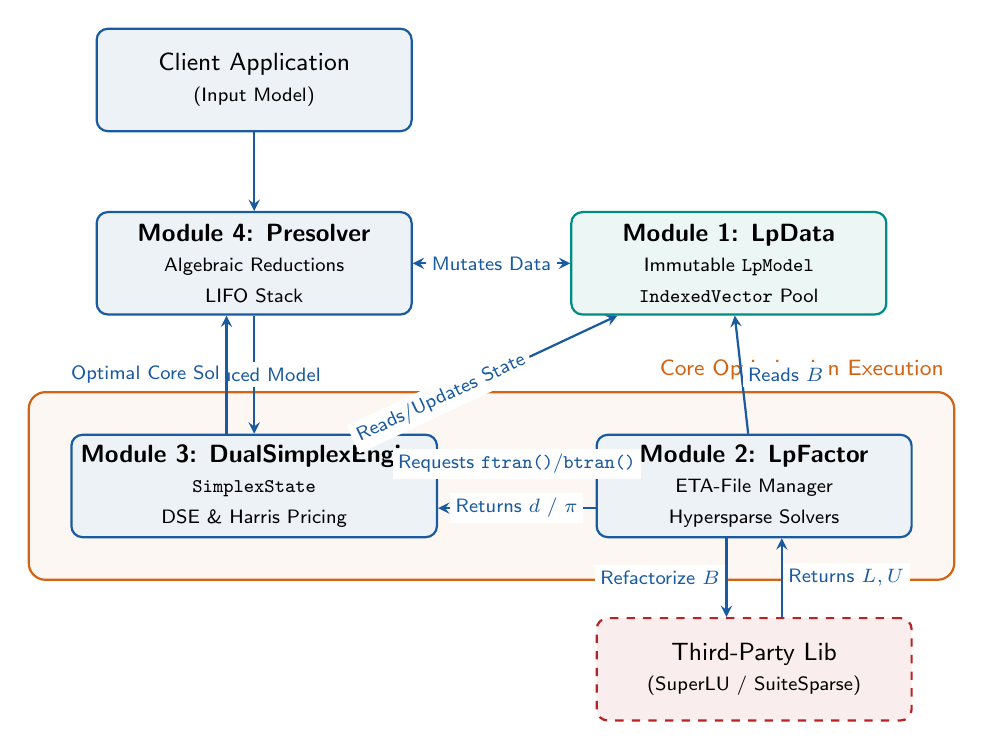
\begin{tikzpicture}[
    node distance=1.5cm and 2cm,
    module/.style={draw=PrimaryBlue, fill=PrimaryBlue!8, thick, rounded corners=4pt, align=center, minimum width=4cm, minimum height=1.3cm, font=\small\sffamily},
    data/.style={draw=AccentTeal, fill=AccentTeal!8, thick, rounded corners=4pt, align=center, minimum width=4cm, minimum height=1.3cm, font=\small\sffamily},
    external/.style={draw=WarnRed, fill=WarnRed!8, thick, dashed, rounded corners=4pt, align=center, minimum width=4cm, minimum height=1.3cm, font=\small\sffamily},
    arrow/.style={->, >=stealth, thick, PrimaryBlue},
    lbl/.style={font=\scriptsize\sffamily, fill=white, inner sep=2pt, text=PrimaryBlue}
]

    % Nodes
    \node[module] (client) {Client Application \\ \scriptsize (Input Model)};
    
    \node[module, below=1cm of client] (presolve) {\textbf{Module 4: Presolver} \\ \scriptsize Algebraic Reductions \\ \scriptsize LIFO Stack};
    
    \node[data, right=2cm of presolve] (datamodel) {\textbf{Module 1: LpData} \\ \scriptsize Immutable \texttt{LpModel} \\ \scriptsize \texttt{IndexedVector} Pool};
    
    \node[module, below=1.5cm of presolve] (simplex) {\textbf{Module 3: DualSimplexEngine} \\ \scriptsize \texttt{SimplexState} \\ \scriptsize DSE \& Harris Pricing};
    
    \node[module, right=2cm of simplex] (factor) {\textbf{Module 2: LpFactor} \\ \scriptsize ETA-File Manager \\ \scriptsize Hypersparse Solvers};
    
    \node[external, below=1cm of factor] (ext) {Third-Party Lib \\ \scriptsize (SuperLU / SuiteSparse)};

    % Background Box for Core Loop
    \begin{scope}[on background layer]
        \node[draw=ExampleOrange, fill=ExampleOrange!5, thick, rounded corners=6pt, fit=(simplex)(factor), inner sep=15pt] (corebox) {};
        \node[anchor=south east, font=\footnotesize\sffamily\color{ExampleOrange}, inner sep=4pt] at (corebox.north east) {Core Optimization Execution};
    \end{scope}

    % Edges
    \draw[arrow] (client) -- (presolve);
    \draw[arrow] (presolve) -- node[lbl] {Reduced Model} (simplex);
    \draw[arrow, transform canvas={xshift=-10pt}] (simplex) -- node[lbl, left] {Optimal Core Sol} (presolve);
    
    \draw[arrow, <->] (presolve) -- node[lbl] {Mutates Data} (datamodel);
    \draw[arrow, <->] (simplex) -- node[lbl, pos=0.3, sloped] {Reads/Updates State} (datamodel);
    \draw[arrow, ->] (factor) -- node[lbl, right] {Reads $B$} (datamodel);
    
    % Core Loop Interaction
    \draw[arrow, transform canvas={yshift=8pt}] (simplex) -- node[lbl] {Requests \texttt{ftran()}/\texttt{btran()}} (factor);
    \draw[arrow, transform canvas={yshift=-8pt}] (factor) -- node[lbl] {Returns $d$ / $\pi$} (simplex);
    
    % External Lib
    \draw[arrow, transform canvas={xshift=-10pt}] (factor) -- node[lbl, left] {Refactorize $B$} (ext);
    \draw[arrow, transform canvas={xshift=10pt}] (ext) -- node[lbl, right] {Returns $L, U$} (factor);

\end{tikzpicture}
\end{center}
\end{document}